\begin{figure}[ht]
\begin{subfigure}{.4\textwidth}
    \centering
    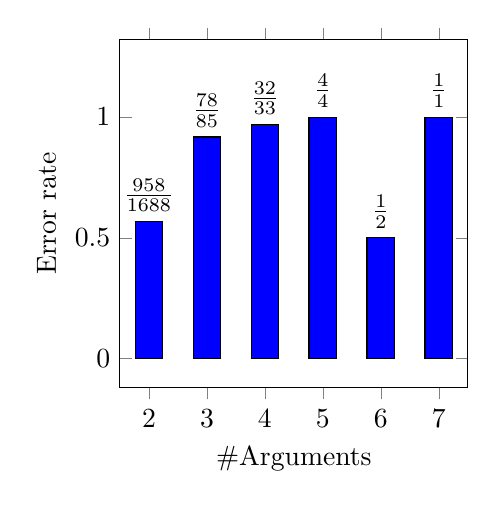
\begin{tikzpicture}
        \begin{axis}[
            enlarge y limits=0.1,
            enlarge x limits=0.1,
            width=6cm,
            height=6cm,
            xtick={2,...,7},
            ymin=0,
            ymax=1.2,
            ybar,
            ylabel=Error rate,
            xlabel=\#Arguments,
            nodes near coords,
            xticklabel style={/pgf/number format/assume math mode},
            yticklabel style={/pgf/number format/assume math mode},
            xtick=data
          ]
            \addplot[ybar,fill=blue,point meta=explicit symbolic] coordinates {
            (2,958/1688) [$\frac{\text{958}}{\text{1688}}$]
            (3,78/85) [$\frac{\text{78}}{\text{85}}$]
            (4,32/33) [$\frac{\text{32}}{\text{33}}$]
            (5,4/4)   [$\frac{\text{4}}{\text{4}}$]
            (6,1/2)   [$\frac{\text{1}}{\text{2}}$]
            (7,1/1)   [$\frac{\text{1}}{\text{1}}$]
            };
        \end{axis}
    \end{tikzpicture}
    \caption{Error rates by the number of arguments each connective has.}
    \label{i:argument-error-len-a}
\end{subfigure}
\begin{subfigure}{.4\textwidth}
    \centering
    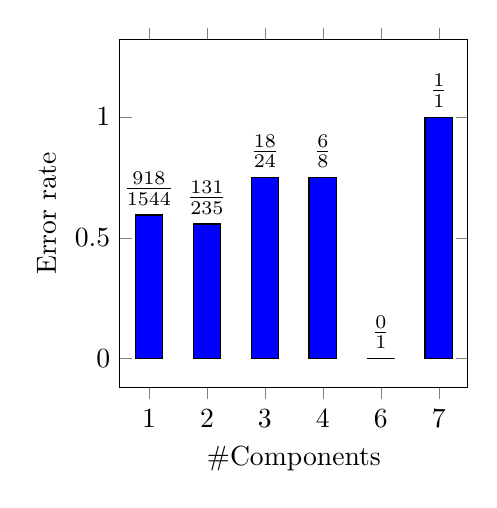
\begin{tikzpicture}
        \begin{axis}[
            enlarge x limits=0.1,
            enlarge y limits=0.1,
            width=6cm,
            height=6cm,
            xticklabels={1,2,3,4,6,7},
            xtick={1,2,...,6},
            ymin=0,
            ymax=1.2,
            ybar,
            ylabel=Error rate,
            xlabel=\#Components,
            nodes near coords,
            xtick=data
          ]
            \addplot[ybar,fill=blue,point meta=explicit symbolic] coordinates {
            (1,918/1544) [$\frac{\text{918}}{\text{1544}}$]
            (2,131/235) [$\frac{\text{131}}{\text{235}}$]
            (3,18/24) [$\frac{\text{18}}{\text{24}}$]
            (4,6/8)   [$\frac{\text{6}}{\text{8}}$]
            (5,0/1)   [$\frac{\text{0}}{\text{1}}$] %6
            (6,1/1)   [$\frac{\text{1}}{\text{1}}$] %7
            };
        \end{axis}
    \end{tikzpicture}
    \caption{Error rates by the number of components each connective has.}
    \label{i:argument-error-len-b}
\end{subfigure}
\begin{subfigure}{1\textwidth}
    \centering
    \vspace{2em}
    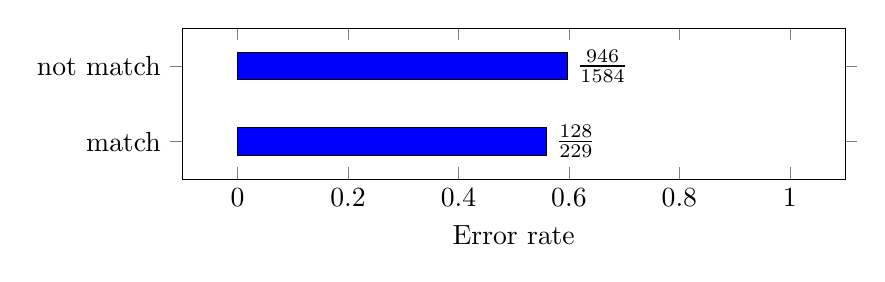
\begin{tikzpicture}
        \begin{axis}[
            enlarge y limits=0.5,
            enlarge x limits=0.1,
            height=3.5cm,
            width=10cm,
            yticklabels={match, not match},
            ytick={1,2},
            xmin=0,
            xmax=1,
            xbar=1pt,
            xlabel=Error rate,
            nodes near coords,
            nodes near coords align={horizontal},
            every node near coord/.append style={
                anchor=west}
            ,
            ytick=data
          ]
            \addplot[xbar,fill=blue,point meta=explicit symbolic] coordinates {
            (128/229,1) [$\frac{\text{128}}{\text{229}}$]
            (946/1584,2) [$\frac{\text{946}}{\text{1584}}$]
            };
        \end{axis}
    \end{tikzpicture}
    \caption{Error rates by whether \#Arguments is the same as \#Components
        in each relation.}
    \label{i:argument-error-len-c}
\end{subfigure}
    \vspace{1em}
    \caption{\label{i:argument-error-len} Error rates for argument extraction
        grouped by different criteria. }
\end{figure}
